%   Include in problem formulation
%   target 2p 
\autsection{Communications for Europa}{Gustavo Feijóo Carrillo}
%   Introductory paragraph
%   Mission Stages and necessary comm links
%       Interplanetary phase

%--> False ref handling
%\iffalse
%(seen on fig. \ref{fig:GalInst1} and \ref{fig:GalInst2})
%\fi

A mission to Europa would be classified as an interplanetary mission, furthermore this one is much more than just that and requires careful considerations of the different scenarios that a mission for Europa's sub-ice ocean exploration requires. First, the interplanetary phase is considered from launch of the spacecraft until Jupiter's orbit insertion (JOI). Second, is the landing phase just after accomplishing EOI (Europa Orbit Insertion), where site determination and certification procedures are carried before the landing of the carrier itself. Third (and most importantly for this writing) is the penetrator release and its descent through the ice crust which requires new development for accomplishing a working communications link through several kilometers of ice. And, at this phase is where the main scientific objectives are to be carried out as well as the majority of all the mission's goals.

%\iffalse
\begin{figure}[htb]
	\centering
	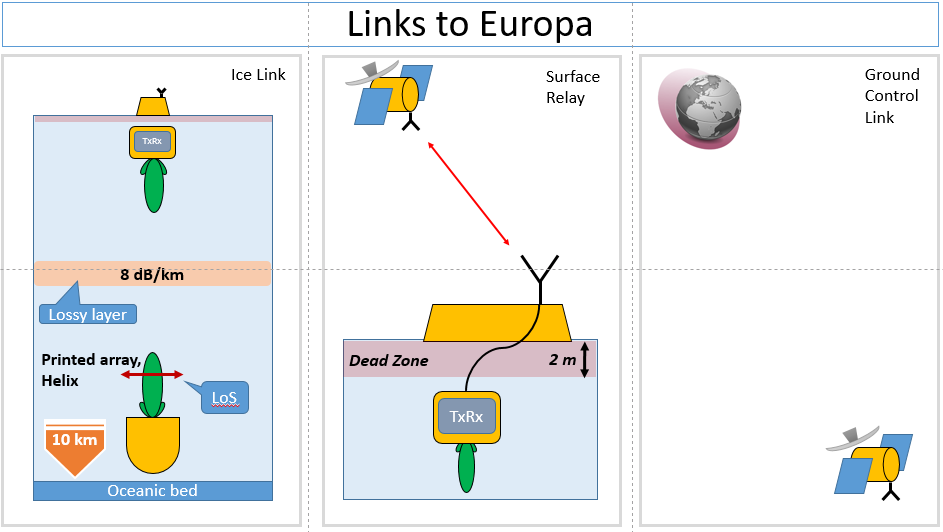
\includegraphics[width=\textwidth]{figures/comms/europaLinks}
	\caption{ \textit{DRAFT} Depiction of the three main stages of a mission to Europa from a telecommunications perspective.}
	\label{fig:europaLinks}
\end{figure}
%\fi

The interplanetary link is feasible thanks to the development of deep space communication networks by ESA (ESTRACK) and NASA (DSN), increasing the reliability of communications and navigation of spacecrafts on missions beyond Earth's orbit. This makes the main hazard during this phase, the high radiation environment of interplanetary space which requires designing for single fault tolerance, a redundant transponder system would be the must straight forward approach. Other problem for this mission stage is the pointing of the antennas since the higher gains needed, increase the requirements for the attitude control systems to keep direct line of sight with ground tracking stations. Universal Space Transponders (UST) are available for down/up-link in UHF with proven capabilities from previous missions to Mars with the inclusion of a down/up-link at X-band and a Ka-band down-link (UHF is TRL-9 and X,Ka-band is TRL-4 according to \cite{clipper}). This leads to focus on the details of a link with a possible Europa orbiter and more important the communications through the ice crust between the penetrator and the lander.


